Nell’ambito di questo progetto è stata scelta l’implementazione di una CNN relativamente standard, eventualmente ampliabile per progetti futuri. Viene utilizzata un modulo di Tensorflow chiamato Keras, grazie al quale possiamo strutturare il modello per poi andare ad analizzare le immagini dei segmenti di iride. 

La funzione che crea il modello è definita in \texttt{model.py} nel pacchetto \texttt{ML\_CNN} e si chiama \texttt{create\_model}.

\begin{minted}
  [
    xleftmargin=\parindent,
    framesep=2mm,
    baselinestretch=1.2,  
    fontsize=\footnotesize,
    linenos,
    breaklines
  ]
  {python}
  
  model = Sequential()
  model.add(Conv2D(layer_size, (3, 3), input_shape=X.shape[1:]))
  model.add(Activation('relu'))
  model.add(MaxPooling2D(pool_size=(2, 2)))

  for l in range(conv_layer - 1):
    model.add(Conv2D(layer_size, (3, 3)))
    model.add(Activation('relu'))
    model.add(MaxPooling2D(pool_size=(2, 2)))

  model.add(Flatten())

  for l in range(dense_layer):
    model.add(Dense(layer_size))
    model.add(Activation('relu'))  

  model.add(Dense(1))
  model.add(Activation('sigmoid'))

  model.compile(loss='binary_crossentropy',
                optimizer='adam',
                metrics=['accuracy'])

  return model, modelname 
\end{minted}

Il tipo di modello che viene utilizzato è quello sequenziale, per creare un modello di questo tipo basta creare un’istanza della classe \texttt{Sequential} di Keras. \texttt{Sequential} è il modo più semplice per costruire un modello, in quanto si definiscono i singoli hidden layers uno ad uno. 

Il primo layer che viene aggiunto è quello convoluzionale, \texttt{Conv2D} (input layer). Esso è a stretto contatto con l’input layer, operando sulle immagini in input, viste come matrici bidimensionali. L’argomento \texttt{layer\_size} indica il numero di neuroni che costituiranno il livello ed è possibile settare questo valore tramite il parametro \texttt{LAYER\_SIZE} della sezione \texttt{NEURAL\_NETWORK\_MODEL} del file di configurazione. Si scelgono solitamente valori standard come 32, 64, 128, etc... in base al numero di immagini presenti nel dataset. Va definita inoltre una kernel size, in questo caso lasciata standard, ovvero 3x3. Essa è la dimensione del kernel, una matrice di filtraggio necessaria alla convoluzione. Una convoluzione è un’operazione che trasforma una funzione matematica al fine di ricavarne maggiori informazioni. In ambito di computer vision, si va a trasformare la matrice rappresentate l’immagine attraverso i valori presenti nel kernel mediante una moltiplicazione matriciale. L’area in cui si trova il kernel viene chiamata receptive field, e in quest’area vengono pian piano applicati i filtri. Questi ultimi non sono definiti in una CNN, in quanto è la rete a imparare in fase di training la tipologia e i parametri di tali filtri. I filtri del layer \texttt{Conv2D} vengono applicati su tutta l’immagine mediante lo “scorrimento” del kernel. La scelta dei filtri che \texttt{Conv2D} applica è inizialmente casuale e basata su distribuzioni conosciute (normale, gaussiana, etc...), ogni filtro viene così trainato in modo differente dagli altri, imparando pian piano a riconoscere features particolari delle immagini. 

Successivamente viene aggiunto un activation layer, un livello che fa passare i dati in input attraverso una funzione di attivazione. Essa è una funzione matematica, possono essere utilizzate diverse funzioni in base al tipo di operazione che si deve effettuare in un determinato layer. Generalmente viene utilizzata la \texttt{RELU (Rectified Linear Unit)} come funzione di attivazione in seguito ad un \texttt{Conv2D} layer. Eventuali diverse funzioni di attivazione verranno citate in seguito.

\begin{figure}[h]
  \centering
  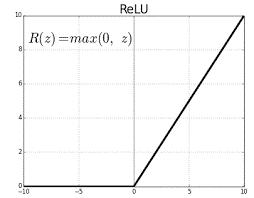
\includegraphics[scale=0.8]{relu.png}
  \caption{Grafico della funzione di attivazione Rectified Linear Unit}
\end{figure}

Viene poi aggiunto un Pooling layer, in particolare un \texttt{MaxPooling2D} layer. La ragione di ciò risiede nel fatto che questo tipo di livello opera un downsampling, riducendo il carico computazionale della rete, senza però perdere le informazioni importanti presenti nell’immagine, le quali vengono poi passate al layer successivo. Con il Max Pooling si considera solo il valore massimo tra tutti i pixel presenti nel kernel del filtro.

\begin{figure}[H]
  \centering
  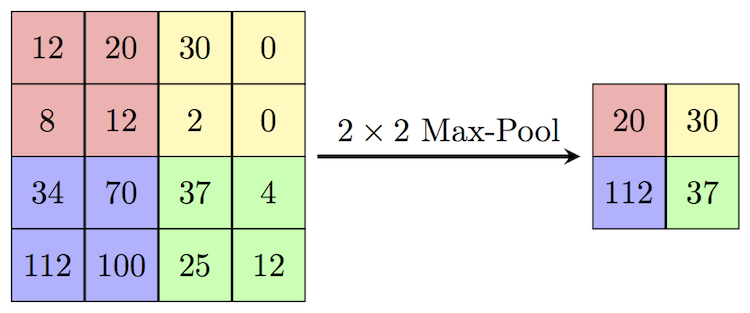
\includegraphics[scale=0.5]{pooling.png}
  \caption{Effetto del layer MaxPooling su un matrice bidimensionale}
\end{figure}

L’utente può poi impostare il valore del parametro \texttt{CONV\_LAYER} che indica il numero di volte in cui la terna di layers sopra descritta (Conv2D-Activation-MaxPooling2D) viene replicata. Così facendo si rende la rete parametrizzata, l’utente ha la possibilità di aggiungere o rimuovere layers intermedi a piacimento. 

Un altro layer molto importante è il \texttt{Flatten layer}. Non necessita di argomenti, in quanto esso si occupa solamente di “appiattire” un insieme di input in un unico vettore monodimensionale contenente tutti gli input. Ad esempio, se l’output del livello precedente ha una shape di (15, 15, 3), un flatten layer crea un vettore monodimensionale (15 x 15 x 3), in modo tale che possa poi essere preso in input da un \texttt{dense layer}. 

Un \texttt{dense layer} è un classico fully connected layer, in quanto ogni neurone è connesso a tutti gli altri. Anche in questo caso l’utente ha libertà di personalizzazione della rete, potendo decidere il numero di dense layers che vengono aggiunti in seguito al flatten layer modificando il parametro \texttt{DENSE\_LAYER}; anche il numero di neuroni dei dense layers è parametrizzabile mediante il parametro precedentemente citato, \texttt{LAYER\_SIZE}. La funzione di attivazione più adatta per questo tipo di layer intermedio rimane la \texttt{RELU}. 

Infine si aggiunge un ultimo \texttt{dense layer} (output layer), il quale si occuperà poi di dare il risultato finale, 0 e 1, essendo il problema in questione di tipo binario; la size di questo layer è 1 essendo che con un unico numero si coprono tutte le classi di categorizzazione (NORMAL e PROBS). La funzione di attivazione questa volta può essere scelta tra \texttt{Sigmoid} e \texttt{Softmax}; entrambe sono funzioni matematiche che si adattano bene al caso d’uso, ma la \texttt{Sigmoid} è scritta appositamente per un caso binario, mentre la \texttt{Softmax} per un caso multiclasse. Nulla sarebbe cambiato scegliendo la \texttt{Softmax} essendo uguali per un caso binario, una è la semplificazione dell’altra. 

\begin{figure}
  \centering
  \begin{subfigure}[b]{0.4\textwidth}
    \centering
    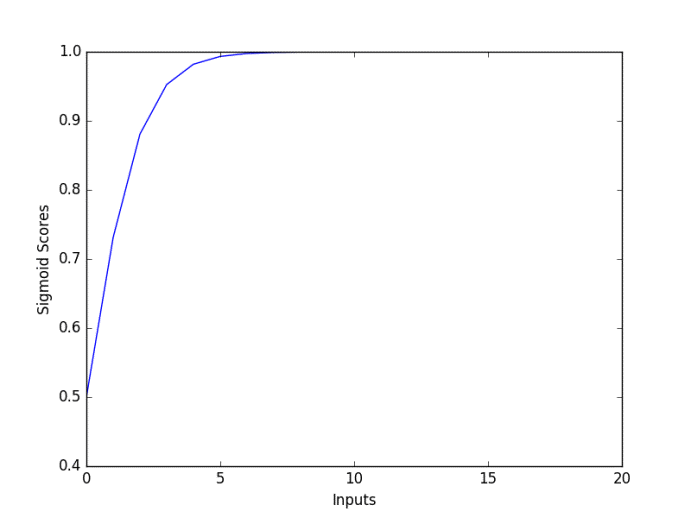
\includegraphics[width=\textwidth]{sigmoid.png}
    \caption{Sigmoid}    
  \end{subfigure}
  \hfill
  \begin{subfigure}[b]{0.4\textwidth}
    \centering
    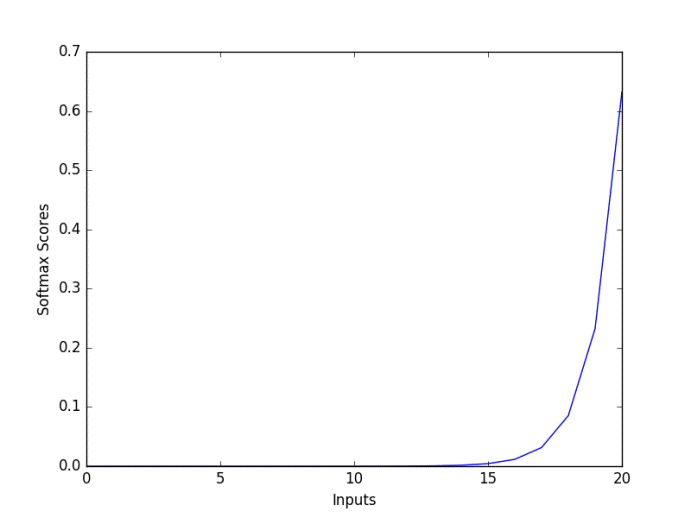
\includegraphics[width=\textwidth]{softmax.png}
    \caption{Softmax}       
  \end{subfigure}
  \caption{Grafici delle due principali funzioni di attivazione per l' ouput layer}
\end{figure}

Si conclude la strutturazione del modello tramite la funzione \texttt{compile} di Keras, la quale configura il modello, preparandolo per la successiva fase di training. I parametri \texttt{loss}, \texttt{optimizer} e \texttt{metrics} scelti sono abbastanza standard per un problema di tipo binario. La funzione di \texttt{loss} è necessaria in quando deve essere costantemente monitorato l’errore dello stato corrente del modello. In questo modo viene analizzato il \texttt{loss rate} in ogni layer, cercando di ridurlo nei layer successivi, aggiustando i pesi utilizzati per le varie operazioni nei livelli. Come metrica viene scelta \texttt{accuracy} in quanto si vuole verificare l’accuratezza del modello in percentuale. Una percentuale alta di \texttt{accuracy} e una bassa di \texttt{loss} indicano che il modello produce risultati attendibili e può essere quindi utilizzato con una buona confidenza per fare predizioni. Il modello viene infine ritornato alla funzione chiamante ed è pronto per la fase di training.
